\usepackage[authoryear,round]{natbib}
\usepackage{multirow}

\newcommand{\sheetnum}{%
	10
}
%\setcounter{section}{\sheetnum-3}
\newcommand{\tutorialtitle}{%
    Support Vector Machines
}
\newcommand{\tutorialtitleshort}{%
	SVM
}
% for slides
\subtitle{\sheetnum \tutorialtitle}

%\maxdeadcycles=1000 % Workaround for ! Output loop---100 consecutive dead cycles because of too many figures

% The following use of algroithms does not work well with the notes:
%
%
%
%
% instead use the following for your algorithms:
%
%\begin{figure}[!t]
%\removelatexerror
%\begin{algorithm}[H]
    % your algo here
    %\label{alg:algolabel}
    %\caption{algocaption}
%\end{algorithm}
%\end{figure}
%\begin{algorithm}
% Below is the definition for the command \removelatexerror:
\makeatletter
\newcommand{\removelatexerror}{\let\@latex@error\@gobble}
\makeatother

\begin{document} %%%%%%%%%%%%%%%%%%%%%%%%%%%%%%%%%%%%%%%%%%%%%%%%%%%%%%%

\sheet{\sheetnum}{\tutorialtitleshort}

\ttopic{\tutorialtitle}

\columnratio{0.2,0.8}\textbf{}
\begin{paracol}{2}
%\setlength{\columnseprule}{0.1pt}
%\setlength{\columnsep}{5em}

\begin{rightcolumn}

% notes version will ignore it
\begin{frame}
\titlepage
\end{frame}

\begin{frame}
\tableofcontents
\end{frame}

\mode<all>
\section{Precursor: Method of Lagrange Multipliers}


\begin{frame}\frametitle{\secname} 
    \begin{center}
    \slidesonly{\huge}
	Don't panic!
    \end{center}
    \begin{center}
        Essentially just hill-climbing (gradient ascent)
    \end{center}
    \pause

\underline{Objective}: \\
\textit{Maximize} an objective function while also satisfying some constraint(s).\\
{
\small(\textit{Maximize}: Find the arguments that maximize an objective function.)
}\\[5mm]
Don't forget: any maximization problem can be turned into a minimization problem\notesonly{ by maximizing the ``negative'' of the function}.
\end{frame}

\subsection{Gradient ascent - unconstrained optimization}
\begin{frame}\frametitle{\subsecname}
Maximize an objective function $f(w_1, w_2)$ (no constraints here).\\
Here $w_1$ and $w_2$ are referred to as free parameters.\\

\begin{figure}[h]
	\centering
	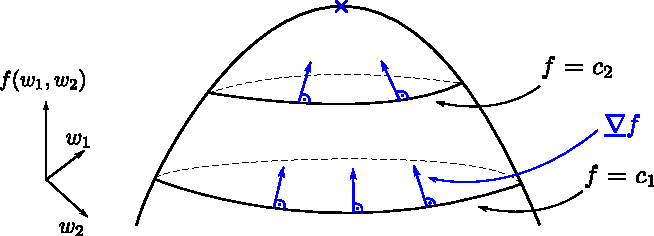
\includegraphics[width=0.8\linewidth]{img/lagrange_objfunction.pdf}
	\mode<article>{
	\caption{
	The objective function $f$ we want to maximize (i.e. reach the blue ${\color{blue}\times}$ at the top). $c_1$ and $c_2$ are level curves where $f$ is constant. 
	The blue arrows indicate the direction of the gradient $\vec \nabla f$, which is always perpendicular to the level curve.
	}
	}
\end{figure}
\slidesonly{
\vspace{-3mm}
}
The gradient $\vec \nabla f$ describes the direction of greatest ascent:\\
\slidesonly{
\vspace{-3mm}
}
\begin{equation}
\vec \nabla f = 
\frac{\partial f}{\partial \vec w} = 
\rmat{\frac{\partial f}{\partial w_1} \\[0.2cm] \frac{\partial f}{\partial w_1} }
\end{equation}

\end{frame}


\newpage

\subsection{Adding a single constraint}
\begin{frame}\frametitle{\subsecname}
We restrict solutions to those that satisfy the constraint $g(w_1, w_2) = c$:

\begin{figure}[h]
\centering
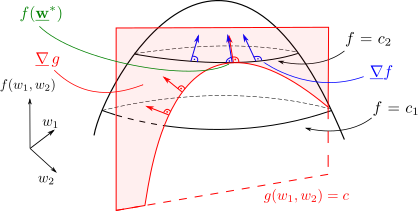
\includegraphics[width=0.7\linewidth]{img/lagrange_objfunction_constrained}
\mode<article>{
\caption{The surface of the constaint cuts through the surface of the objective function. The highest point that can be reached on $f$ which also intersects with $g$ is unique in that the gradients of $f$ and $g$ both point in the same direction with only a difference in scale.}
}
\end{figure}

\only<1,2>{
\question{What is characteristic of the solution to the constrained optimization problem?}\\
}
\notesonly{
-The solution of the constrained optimization problem is characterized by:
}
\only<2>{
\slidesonly{\vspace{-5mm}}
\begin{equation}
    \vec \nabla f = \lambda' \vec \nabla g\,,\quad
\text{where $\lambda'$ is a scaling factor.}
\label{eq:equality}
\end{equation}
}
\notesonly{\eqref{eq:equality} holds for the highest position in $f$ while also satisfying the constraint.\\

Consequently,}
% temporarily change footnote marks to symbols so not to confuse with exponents
\renewcommand*{\thefootnote}{\fnsymbol{footnote}}
\only<3>{
\slidesonly{\vspace{-5mm}}
\begin{align}
  \vec \nabla f \; - \lambda' \vec \nabla g     &= \vec 0 \\
  \vec \nabla f \; + \underbrace{(- \lambda')}_{=:\lambda} \vec \nabla g &= \vec 0 \\
  \vec \nabla f \;  + \lambda \vec \nabla g      &= \vec 0\notesonly{\;\footnotemark }
  \label{eq:equalitylambda}
\end{align}
}
\notesonly{
    \footnotetext{
    The switch from $\lambda'$ to $\lambda$ is to be more consistent with lecture slides.
    }
}
% change footnote marks back to original scheme (numbers)
\renewcommand*{\thefootnote}{\arabic{footnote}}

\end{frame}

\begin{frame}
\only<1,2>{
The constrained optimization problem is formulated as:
\begin{equation}
\underbrace{f(w_1, w_2) \;\eqexcl\; \max_{w_{1},w_{2}}}_{\text{maximization}} \quad  \text{subject to} \quad \underbrace{g(w_1,w_2)\;-c\; = \; 0}_{\text{a single constraint}}
\label{eq:optconstrained}
\end{equation}
}
\notesonly{
The \emph{Lagrangian} function reformulates the constrained optimization problem from \eqref{eq:optconstrained} in a way that reflects the relationship of the two gradients at the solution and thus facilitate finding the solution \eqref{eq:equalitylambda}.} The \emph{Lagrangian} is \notesonly{therefore }defined as:

\only<2,3>{
\begin{equation}
L(w_1, w_2, \lambda) \; = \; f(w_1,w_2) + \lambda(g(w_1, w_2)-c)
\end{equation}

Setting the gradient $\nabla L$ to zero guarantees $\vec \nabla f \;  + \lambda \vec \nabla g = \vec 0$
}
\only<3>{

\begin{equation}
\vec \nabla L = 
\rmat{
	\frac{\partial L}{\partial w_1} \\[0.5cm]
	\frac{\partial L}{\partial w_2} \\[0.5cm]
	\frac{\partial L}{\partial \lambda}
	}
=
\rmat{
	\frac{\partial f}{\partial w_1} \quad+\quad \lambda \frac{\partial g}{\partial w_1} \\[0.3cm]
	\frac{\partial f}{\partial w_2} \quad+\quad \lambda \frac{\partial g}{\partial w_2} \\[0.3cm]
	\underbrace{\frac{\partial f}{\partial \lambda}}_{=0} \;+\; g(w_1, w_2)-c
	}
=
\rmat{
	0 \\[0.5cm]
	0 \\[0.5cm]
    0
	}
= \vec 0
\label{eq:lagrangiangrad}
\end{equation}

Setting the first two elements of $\nabla L$\notesonly{, namely $\frac{\partial L}{\partial w_1}$ and $\frac{\partial L}{\partial w_2}$,} to zero ensures that $\nabla f = -\lambda \nabla g$,\\
while $\frac{\partial L}{\partial \lambda}=0$ ensures that $g(w_1, w_2) = c$.\\

\notesonly{\eqref{eq:lagrangiangrad} describes a system of }3 equations with 3 unknowns.\notesonly{
\footnote{
Not much emphasis is put on knowing how to solve this by hand. If interested, the wikipedia article on \href{https://en.wikipedia.org/wiki/Lagrange_multiplier\#Examples}{Lagrange multiplier} provides some examples.}
}\\

We refer to $\lambda$ as the \emph{multiplier} for the constraint $c$.
}
\end{frame}

\subsection{Multiple constraints}

\begin{frame}
 
\question{How do we extend this to multiple {\color{red}{equality}} constraints?}

\slidesonly{\vspace{-2mm}}
    
\begin{equation}
\underbrace{f_0(\vec w) \;\eqexcl\; \text{max}}_{\text{maximization}} \quad  \text{and} \quad f_k(\vec w)\;{\color{red}{=}}\; \; 0 \;, \quad k = 1,\ldots,m
\label{eq:optimizationequalitymultipe}
\end{equation}

where $m$ denotes the number of constraints. $f_{0}(\vec w)$ is reserved for the function to be optimized., while $f_{1}(\vec w), f_{2}(\vec w),\ldots,f_{m}(\vec w)$ is used for all $m$ constraints.

The Lagrangian for multiple constraints is defined as:
%\slidesonly{\vspace{-2mm}}
\begin{align}
L(\,\vec w\;, \overbrace{\{\lambda_k\}}^{
\mathclap{
\substack{\text{a multiplier} \\
\text{for each constraint}}
}
}) 
\; &= \; 
f_0(\vec w) + \lambda_1 \, f_1(\vec w) + \lambda_2 \, f_2(\vec w) + \, \ldots \, + \lambda_m \, f_m(\vec w) \\
\; &= \; 
f_0(\vec w) + \sum_{k=1}^{m} \lambda_k \, f_k(\vec w)
\label{eq:lagrangianmultiple}
\end{align}

\question{What if we have {inequality} constraints?}

\end{frame}

\begin{frame}

In the case of {\color{red}{inequality}} constraints, our constrained optimization problem would have the following form:

\begin{equation}
\underbrace{f_0(\vec w) \;\eqexcl\; \text{max}}_{\text{maximization}} \quad  \text{and} \quad f_k(\vec w)\; {\color{red}{\le}} \; 0 \;, \quad k = 1,\ldots,m{}
\label{eq:optimizationINequalitymultipe}
\end{equation}

However, the Lagrangian remains the same\notesonly{ as in \eqref{eq:lagrangianmultiple}}. The inequality is taken into account in that the solutions for $\lambda$ extend to some range:

\begin{equation}
L(\,\vec w\;, \{\lambda_k\}
) \; = \; f_0(\vec w) + \sum_{k=1}^{m} \lambda_k \, f_k(\vec w)\,,\qquad
\lambda_{k} \;{\color{red}{\ge}}\; 0 \quad \forall k \in \{1,\ldots,m\}
\label{eq:lagrangianINequalitymultiple}
\end{equation}
 
    
\end{frame}

\mode*

\mode<all>
\section{Maximum Margin Classifiers}

\mode<presentation>{
\begin{frame} 
    \begin{center} \huge
        \secname
    \end{center}
    \begin{center}
     What is a \emph{margin} and why should we care about maximizing it?   
    \end{center}
\end{frame}
}

\subsection{Identifying the margin}

\begin{frame}\frametitle{\subsecname}
\mode<article>{
Consider the following linearly separable binary classification problem and the different hyperplanes for separating the two classes. In order to identify the margn of a hyperplane:
}

\only<1-3>{
\begin{enumerate}[(a)]
\item select a hyperplane,
\item select the training point closest to the hyperplane. Call it $\vec x^{*}$. \notesonly{$\vec x^{*}$ has the shortest normal distance to the hyperplane.}
\item measure the normal distance between $\vec x^{*}$ and the hyperplane and call it $\mathrm{d}_{w}$
\end{enumerate}
}
%\begin{figure}[h]
    %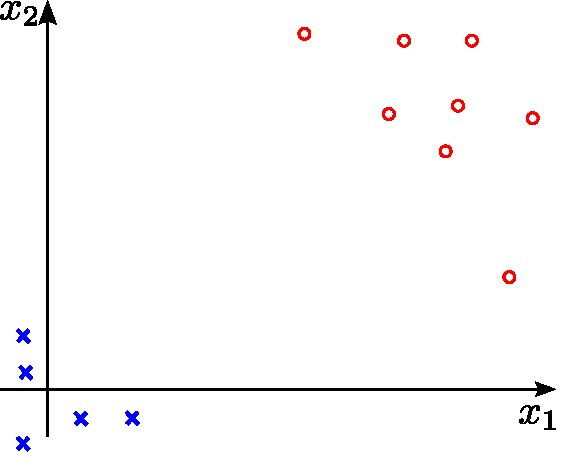
\includegraphics[width=0.5\linewidth]{img/section2_fig13_v2_nomargin_h_none}
    %\mode<article>{
    %\caption{Different hyperplanes for a linearly separable problem.}
    %}
%\end{figure}

\begin{figure}[ht]
     \centering
     \savebox{\imagebox}{
	 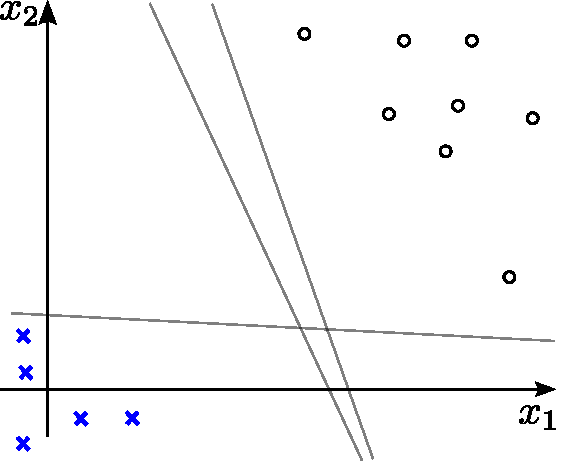
\includegraphics[width=0.35\textwidth]{img/section2_fig13_v2_nomargin_h_multiple}}%
     \only<1>{
     \begin{subfigure}[t]{0.35\textwidth}
         \centering
         \usebox{\imagebox}% Place largest image
         \mode<article>{
         \caption{}
         }
         \label{fig:multiplehyperplanes}
     \end{subfigure}
     }
     \hspace{2mm}
     \only<2>{
     \begin{subfigure}[t]{0.35\textwidth}
         \centering
         \raisebox{\dimexpr.5\ht\imagebox-.5\height}{% Raise smaller image into place
         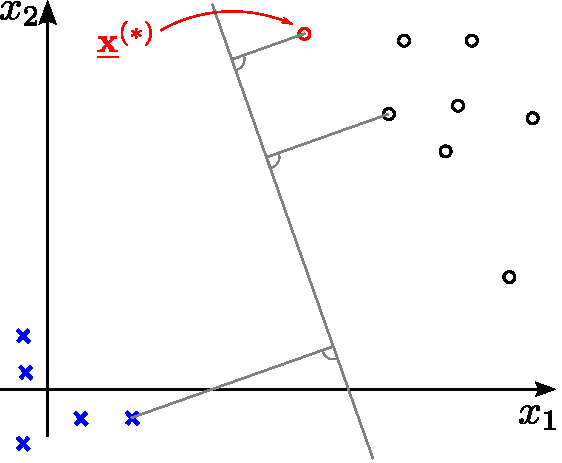
\includegraphics[width=0.99\textwidth]{img/section2_fig13_v2_nomargin_h_closest}
         }
         \mode<article>{
         \caption{}
         }
     \end{subfigure}
     }
     \hspace{2mm}
     \only<3,4>{
     \begin{subfigure}[t]{0.35\textwidth}
         \centering
         \raisebox{\dimexpr.5\ht\imagebox-.5\height}{% Raise smaller image into place
         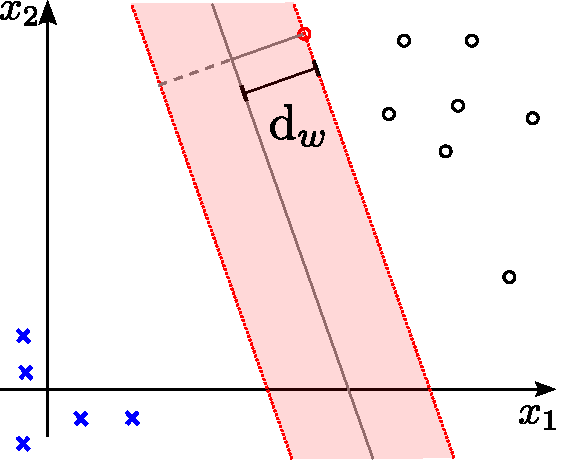
\includegraphics[width=0.99\textwidth]{img/section2_fig13_v2_nomargin_h_margin}
         }
         \mode<article>{
         \caption{}
         }
         \label{fig:margin}
     \end{subfigure}
     \hspace{2mm}
     }
     \only<4>{
     \begin{subfigure}[t]{0.35\textwidth}
         \centering
         \raisebox{\dimexpr.5\ht\imagebox-.5\height}{% Raise smaller image into place
         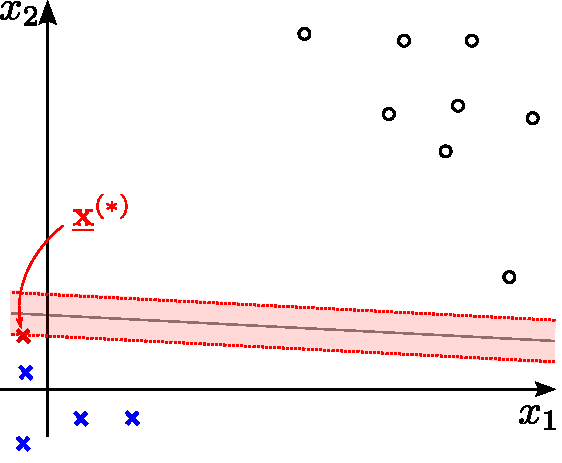
\includegraphics[width=0.99\textwidth]{img/section2_fig13_v2_nomargin_h_marginother}
         }
         \mode<article>{
         \caption{}
         }
         \label{fig:marginother}
     \end{subfigure}
     }
     \mode<article>{
     \caption{Identifying the margin $\mathrm{d}_{w}$ for a hyperplane.}
	 }
	 \label{fig:identifymargin}
\end{figure}
\only<3>{
The distance $\mathrm{d}_{w}$ is the \emph{margin} for that hyperplane.
}
\only<4>{

\question{What are the implications of a wide vs. narrow margin?}

}
    
\end{frame}

\begin{frame}\frametitle{Wide vs. narrow margins}
 
Remember: We are only dealing with a linearly separable problem.


	\begin{figure}[h]
		\centering
		\slidesonly{
		\only<1>{
		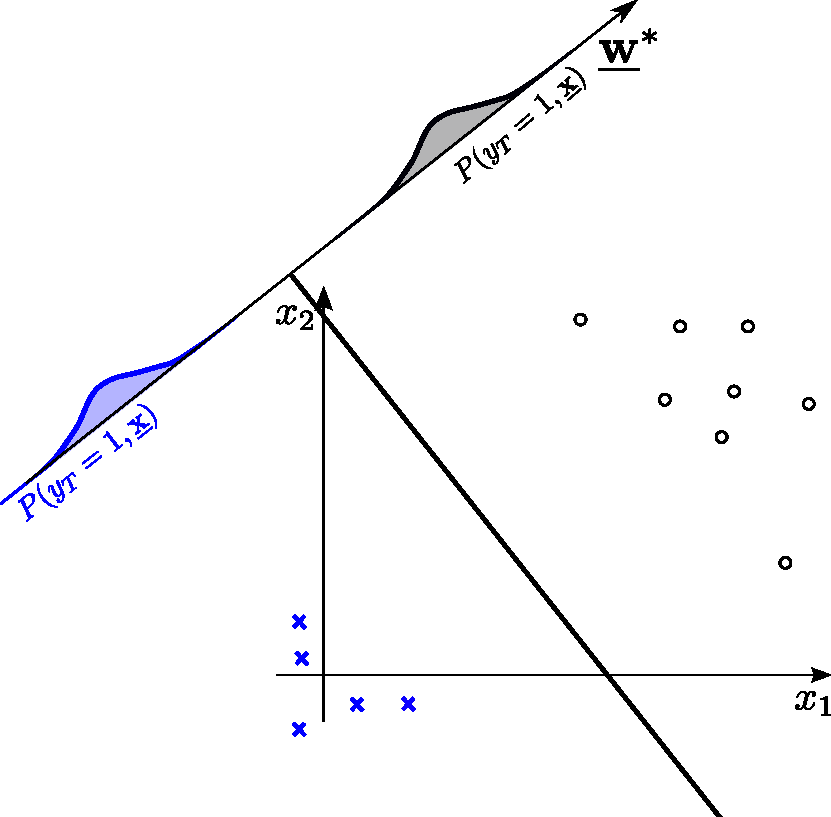
\includegraphics[height=4.5cm]{img/section2_fig13_v2_nomargin_h_distr} 
		}
		}
		\only<2>{
		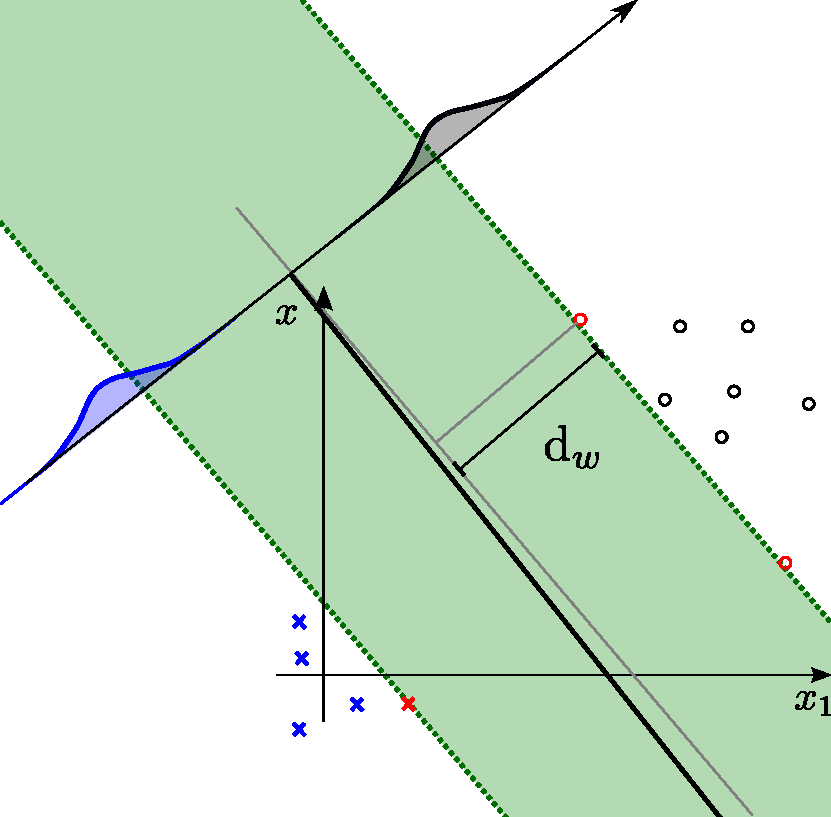
\includegraphics[height=4.5cm]{img/section2_fig13_v2_nomargin_h_margin_max} 
		}
		\mode<article>{
		\caption{
		Potential generalization abilities with maximum margin.
		}
		\label{fig:conditionsv}
		} 
	\end{figure}
 
\mode<article>{
      The {\em margin} is the smallest distance between a separating hyperplane and a training sample. The training sample closest to the decision boundary is denoted with $\vec x^{(*)}$.\\
            Separating the training data with a larger margin is more likely to reduce classification error on unseen data (i.e. lower generalization error, less overfitting).
            A simplistic justification for this: \\
            Assume we have found the separating hyperplane with the maximum margin for perfectly separable data. From this:
            \begin{enumerate}[(1)]
                \item The distance between the classes is at least twice as wide as the distance from the hyperplane to $\vec x^{(*)}$ (i.e. $2 \mathrm{d}_{w}$).
                \item An unseen pattern $\vec x^{(test)}$ is more likely to land closer to training patterns of the same class than patterns from the other class.
                \item The distance between $\vec x^{(test)}$ and $\vec x^{(*)}$ is more likely to be 
                \begin{itemize}
                 \item \emph{larger} than the margin, if the points belong to \emph{different} classes and more likely to be 
                 \item \emph{below} the margin, if both belong to the \emph{same} class.
                 \end{itemize}
            \end{enumerate}
            Another way to look at this:\\
            
            Consider a second hyperplane with the same orientation $\vec w$ but less than maximum (i.e. more narrow) margin. Shift the second hyperplane so that our sample $\vec x^{(*)}$ also lies on the margin of the second hyperplane. The shifting results in the decision boundaries of both hyperplanes appearing parallel to one another, both make contact with $\vec x^{(*)}$. The difference is that the hyperplane with the smaller margin appears to lie inside the first hyperplane. Now consider an unseen pattern $\vec x_{(test)}$ that is very similar to $\vec x^{(*)}$ (i.e. $\vec x_{(test)} = \vec x^{(*)} + \vec {noise}$). $\vec x_{(test)}$ belongs to the same class as $\vec x^{(*)}$. The noise can result in the $\vec x_{(test)}$ falling inside the margin of the first hyperplane. Because the margin of the second hyperplane is more narrow, the decision boundary of that plane is closer to $\vec x^{(*)}$. This means that $\vec x_{(test)}$ is more likely to fall on the wrong side of the second decision boundary and get misclassified (i.e. higher generalization error). This is less likely to happen for the first hyperplane because the maximum margin pushes the decision boundary away from the $\vec x^{(*)}$. We would need to apply more noise on $\vec x_{(test)}$  until it gets misclassified by the maximum margin hyperplane.\vspace{5cm}
            
}
\only<2>{
        \notesonly{Another implication of the maximizing the margin is that}\slidesonly{Also,} the optimal hyperplane with maximum margin is a \emph{unique} solution to the optimization problem.
    }
    
\end{frame}

\subsection{Margins and the VC-dimension}

\begin{frame}

\slidesonly{\vspace{-5mm}} 

\question{Where does the VC dimension come into all of this?}\\

\slidesonly{\vspace{-5mm}} 

\begin{equation}
\, \uparrow \text{margin} \;\; \leadsto \;\; \dvc \, \downarrow   
\end{equation}

\mode<article>{
\begin{figure}[h]
    \centering
    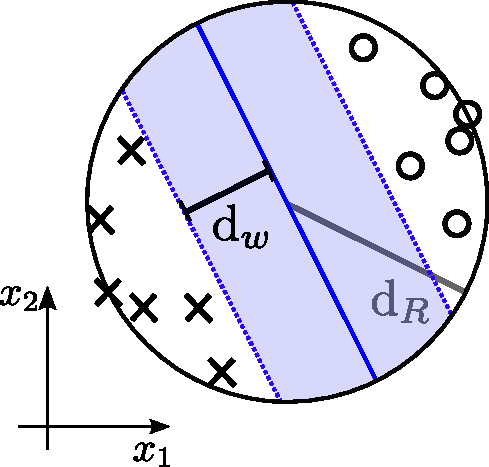
\includegraphics[height=4cm]{img/dvc_margin1} 
    \mode<article>{
    \caption{
    The general setting assumed for deriving the upper bound on the VC-dimension of the maximum margin classifier.
    }
    \label{fig:dvcmarginboundsetting}
    } 
\end{figure}
}
\mode<presentation>{
\placeimage{11.}{6.5}{img/dvc_margin1}{width=3.5cm}
}

\notesonly{        
Large margins imply a small VC dimension. }A larger margin tightens the upper bound of the VC dimension, regardless of the dimensionality of the problem. 

\begin{block}{\textit{Theorem 10.3} in \citep{Vapnik1998}}
\notesonly{states that}

\begin{equation}
    \dvc \quad\leq\quad \min \bigg( \bigg\lfloor 
    \frac{\mathrm{d}_R^2}{\mathrm{d}_{{w}}^2}
\bigg\rfloor, N \bigg) + 1\slidesonly{\qquad\qquad}
\label{eq:dvcmarginbound}
\end{equation}

where,\\

\begin{tabular}{rl}
    $N$\;:& dimension of feature space \\[1mm]
    $\mathrm{d}_w$\;:& the margin: 
        $\frac{1}{\|\vec w \|} \geq \mathrm{d}_w$ \\[1mm]
    $\mathrm{d}_R$\;:& radius of a sphere containing all training points.\\
    &It quantifies the support of $\vec x$:\\
    & $P(\vec x) \neq 0$ for $\|\vec x\| \leq \mathrm{d}_R$ (i.e. no points exist outside of this sphere.)
\end{tabular}
\end{block}

\mode<article>{

The bound in \eqref{eq:dvcmarginbound} assumes a setting as depicted by \figref{fig:dvcmarginboundsetting}. It tells us that, if we draw a sphere around our training data with radius $\mathrm{d}_{R}$ and a second sphere inside of it using the margin $\mathrm{d}_{w}$ as its radius, knowing that the inner sphere is placed in the center and does not contain any datapoints, the theorem then tells us that the VC-dimension is no longer $N+1$ but only as big as the integer component
\footnote{If interested in a proof for \textit{Theorem 10.3}, see 
\href{http://web.eecs.umich.edu/\~jabernet/eecs598course/fall2015/web/notes/lec11\_101315.pdf}
{http://web.eecs.umich.edu/\~jabernet/eecs598course/fall2015/web/notes/lec11\_101315.pdf}
}
\footnote{According to \citep{hush2001vc}, it is debatable whether one should apply $\lfloor \cdot \rfloor$ (floor) or $\lceil \cdot \rceil$ (ceil operation) while pointing out that the latter is possibly incorrect but ``asymptotically sharper'' with reference to \citep{Burges1998}.}
on the ratio $\frac{\mathrm{d}_R^2}{\mathrm{d}_{{w}}^2}$.

}




% illustrations adapted from http://www.cs.columbia.edu/~jebara/4771/notes/class5x.pdf

\mode<article>{
To illustrate:
}

\end{frame}

\begin{frame}\frametitle{\subsecname}

Recall the definition of the $\dvc$ as the \underline{maximal number of training points $p$} that a model can \emph{shatter}.\\

\only<1>{
\begin{figure}[h]
     \centering
     \savebox{\imagebox}{
	 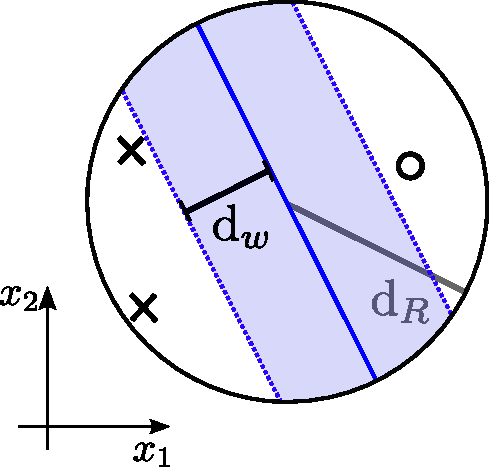
\includegraphics[width=0.22\textwidth]{img/dvc_margin_3pts0}}%
     \begin{subfigure}[t]{0.22\textwidth}
         \centering
         \usebox{\imagebox}% Place largest image
         \mode<article>{
         \caption{}
         }
     \end{subfigure}
     \hspace{2mm}
     \begin{subfigure}[t]{0.22\textwidth}
         \centering
         \raisebox{\dimexpr.5\ht\imagebox-.5\height}{% Raise smaller image into place
         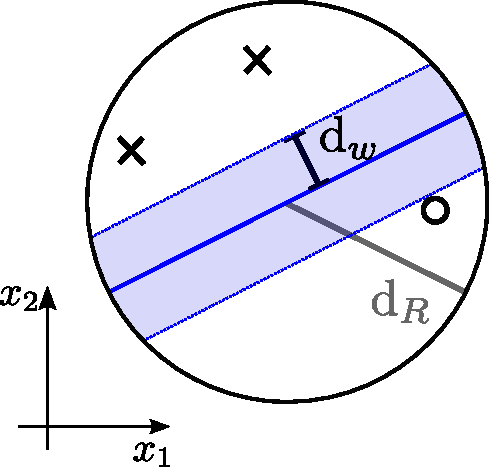
\includegraphics[width=0.99\textwidth]{img/dvc_margin_3pts1}
         }
         \mode<article>{
         \caption{}
         }
     \end{subfigure}
     \hspace{2mm}
     \begin{subfigure}[t]{0.22\textwidth}
         \centering
         \raisebox{\dimexpr.5\ht\imagebox-.5\height}{% Raise smaller image into place
         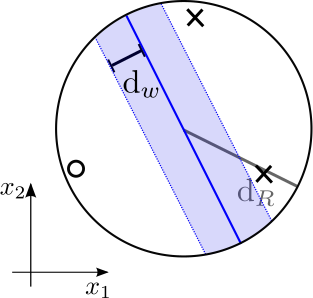
\includegraphics[width=0.99\textwidth]{img/dvc_margin_3pts2}
         }
         \mode<article>{
         \caption{}
         }
     \end{subfigure}
     \mode<article>{
     \caption{A linear neuron can shatter any label configuration of 3 points regardless of how they are arranged in 2D space (excluding colinear points).}
	 }
	 \label{fig:shatter3pts}
\end{figure}

Therefore, $\dvc = N+1 = 3$, for a linear classifier with a margin $0\,\le\,\mathrm{d}_{w}\,<\,\mathrm{d}_{R}$.
}
\only<2>{
As the margin increases, i.e. $\mathrm{d}_{w}\,\rightarrow\,\mathrm{d}_{R}$\notesonly{, $\dvc$ of the linear classifier drops from $N+1$ to $1+1=2$ (e.g. from 3 to 2).}
\slidesonly{
$$
\dvc\;\rightarrow\;2
$$}
In the case of $\mathrm{d}_{w} = \mathrm{d}_{R}$\notesonly{ the VC-dimension will be reducedto 1. But since this implies a dataset of only a single point, it is not such an interesting case.}
\slidesonly{
$$
\dvc\;\rightarrow\;1
$$}


\begin{figure}[h]
     \centering
     \savebox{\imagebox}{
	 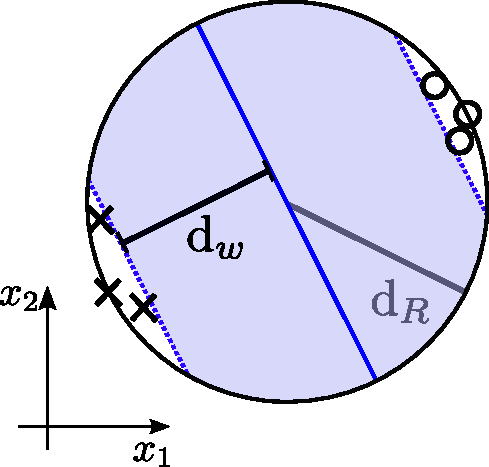
\includegraphics[width=0.22\textwidth]{img/dvc_margin0}}%
     \begin{subfigure}[t]{0.22\textwidth}
         \centering
         \usebox{\imagebox}% Place largest image
         \mode<article>{
         \caption{}
         }
     \end{subfigure}
     \hspace{2mm}
     \begin{subfigure}[t]{0.22\textwidth}
         \centering
         \raisebox{\dimexpr.5\ht\imagebox-.5\height}{% Raise smaller image into place
         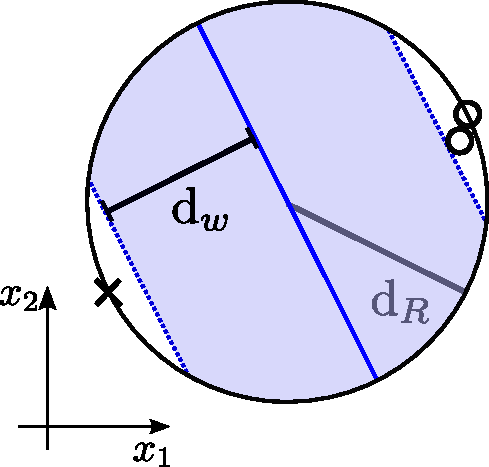
\includegraphics[width=0.99\textwidth]{img/dvc_margin_large}
         }
         \mode<article>{
         \caption{}
         }
     \end{subfigure}
     \hspace{2mm}
     \begin{subfigure}[t]{0.22\textwidth}
         \centering
         \raisebox{\dimexpr.5\ht\imagebox-.5\height}{% Raise smaller image into place
         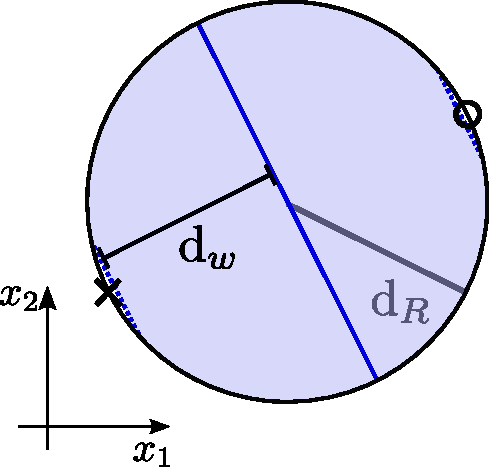
\includegraphics[width=0.99\textwidth]{img/dvc_margin_max}
         }
         \mode<article>{
         \caption{}
         }
     \end{subfigure}
     \mode<article>{
     \caption{A linear neuron can no longer shatter $N+1$ points when the margin is maximal.}
	 }
	 \label{fig:shatter3pts}
\end{figure}
}
     
            
            
\end{frame}

\begin{frame}
\only<1,4>{
If the margin provides a bound for the $\dvc$
}
\only<1,4>{
\mode<presentation>{ 
$$
    \dvc \quad\leq\quad \min \bigg( \bigg\lfloor 
    \frac{\mathrm{d}_R^2}{\mathrm{d}_{{w}}^2}
\bigg\rfloor, N \bigg) + 1\slidesonly{\qquad\qquad}
$$
}
}
\only<1->{

\question{What were the benefits of reducing $\dvc$?}

%leave line break for effective pause
}
\only<2,3>{
Recall\notesonly{ that one of the key results of Statistical Learning Theory was the formulation of the bound on the generalization error, given a finite set of samples:}
\notesonly{
\begin{equation}
    P \bigg\{ \sup_{\vec{w} \in \Lambda} \Big| R_{[\vec w]} 
        - R_{\emp [\vec{w}]}^{(p)} \Big| > \eta \bigg\} 
    < 4 \exp \Big( G_{(2p)}^\Lambda - p 
        \big( \eta - \smallfrac{1}{p} \big)^2 \Big)
    \eqexcl \epsilon
\end{equation}

where $\Lambda$ denotes the model class and $G^{\Lambda}_{(2p)}$ denotes the growth function\footnote{cf. lecture 2.1.3 on Statistical Learning Theory and corresponding notes.}.
}

With a probability larger than $\,1 - \epsilon\,$ we obtain:

\begin{equation}
    R_{[\vec w]} < \underbrace{R_{\emp [\vec{w}]}^{(p)}
        }_{\substack{\text{empirical}\\\text{error}}} +
        \underbrace{\bigg(
        \smallfrac{G_{(2p)}^\Lambda - \ln \frac{\epsilon}{4}}{p}
        \bigg)^{\frac{1}{2}} \,+\, \frac{1}{p}
        }_{\text{complexity term}~C(p,\dvc)}
        \label{eq:generalizationresultsriskgrowth}
\end{equation}

\notesonly{For a given $\epsilon$, the complexity term
only depends on $p$ and $\dvc$.}}
\mode<article>{
 Therefore, the VC dimensions helps in formulating a bound on the \textbf{generalization ability} of Empirical Risk Minimization (ERM). 
 Knowing that 
 }
 \only<2,3>{
 \begin{itemize}
  \notesonly{\item the risk $R_{[\vec w]}$ and empirical risk $R_{\text{emp}[\vec w]}$ are represented by the generalization $E^{G}_{[\vec w]}$ and training error $E^{T}_{[\vec w]}$, respectively:\\
  $R_{[\vec w]} \, \corresponds \, E^{G}_{[\vec w]}\,,$
  $
  R_{\text{emp}[\vec w]}  \, \corresponds \, E^{T}_{[\vec w]}
  $
  and that} 
  \item for $p>\dvc$:
  $$G^{\Lambda}_{(p)} \le \dvc \Big(\ln \frac{p}{\dvc} + 1\Big)\,,$$
  \end{itemize}
  }~\notesonly{
\eqref{eq:generalizationresultsriskgrowth} can be reformulated in order to  highlight the relationship between the VC dimension and the generalization ability of the model class:}\\

\notesonly{For a finite training set, the generalization error is bound with probability $1-\epsilon$:}
\only<4,5>{
\slidesonly{\vspace{-7mm}}
\begin{equation}
    E^{G}_{[\vec w]} \;\le\; E^{T}_{[\vec w]} + 
    \underbrace{
    \sqrt{\frac{\dvc \left(\ln \frac{2\,p}{\dvc} + 1\right)-\ln\frac{\epsilon}{4}}{p}}}_{\text{generalization gap}} + \frac{1}{p} \quad \text{for } p > \dvc
    \label{eq:generalizationresults}
\end{equation}

\question{What about $\dvc \rightarrow 0$? Is this ideal?}

%\begin{equation}
%\boxed{
%\;
%\uparrow \, \text{margin}
%\quad \leadsto \quad
%\dvc \, \downarrow 
%\;   
%}
%\end{equation}  
}

\only<5>{
\begin{figure}[h]
    \centering
    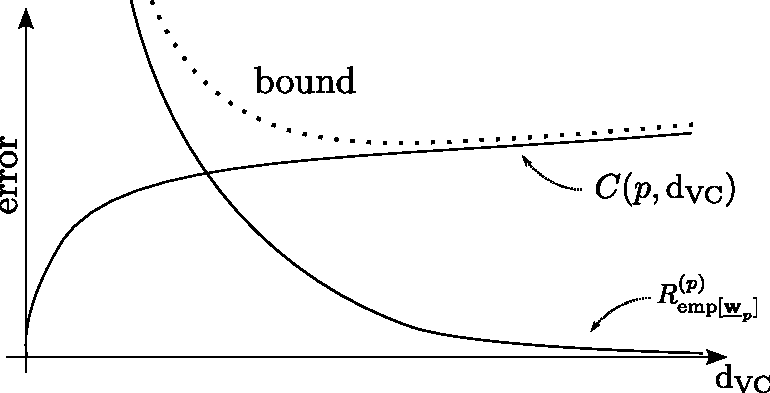
\includegraphics[height=3.5cm]{img/section2_fig12_v2} 
    \mode<article>{
    \caption{
    The effect of the VC-dimension and bias-variance trade-off
    }
    \label{fig:dvcbiasvariance}
    } 
\end{figure}

}

\end{frame}



\mode*

\mode<all>
\section{The Support Vector Machine (SVM)}

\mode<presentation>{
\begin{frame} 
    \begin{center} \huge
        \secname
    \end{center}
    \begin{center}
     Finding the separating hyperplane with maximum margin\\+ the ``kernel trick''   
    \end{center}
\end{frame}
}

\subsection{SVMs are Maximum Margin Classifiers}

\begin{frame}\frametitle{The binary classification setting}

\mode<article>{
The binary classification setting:\\

\begin{figure}[h]
    \centering
    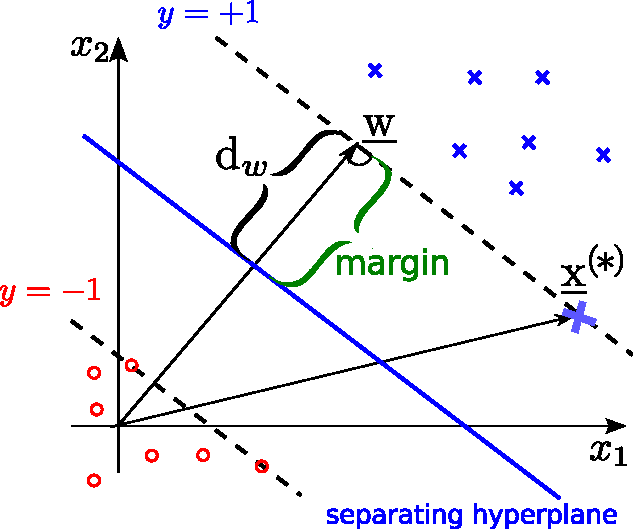
\includegraphics[height=4cm]{img/section2_fig13_v2_space} 
    \mode<article>{
    \caption{
    Binary classification setting.
    }
    \label{fig:setting}
    } 
\end{figure}
}
\mode<presentation>{
\placeimage{8.7}{2.5}{img/section2_fig13_v2_space}{width=5.2cm}
}


\begin{itemize}
	\item \underline{Data}:\\[2mm]
	$
	\Big\{ \left(\vec x^{(\alpha)}, y^{(\alpha)}_{T} \right) \Big\}_{\alpha=1}^{p}\,
	$\\[2mm]
	where $\vec x \in \R^{N}$, $y_T^{(\alpha)} \in \{-1, 1\}$\\

	\item \underline{Model}:\\[2mm]
	$
	y(\vec x; \vec w) = \sign \big( \vec w^{\top} \vec x + b \big)
	$
    
    \item \underline{Objective}:
    
    Choose the decision boundary s.t. the margin is \emph{maximal}.
    
    \item \underline{Assumption}:
    
    Perfect linear separation of both classes:
    
    In the case of a simple connectionist neuron:
    \begin{equation}
    \vec w^{\top} \vec x + b \;\;
    \left \{ \begin{array}{ll}
					\ge& 0 \;\;\text{for } {\color{blue}y_{T} = +1}\\
					<& 0 \;\;\text{for } {\color{red}y_{T} = -1}
				\end{array} \right.  
    \end{equation}
    The solution is not unique.
    
\end{itemize}
    
\end{frame}

\begin{frame}\frametitle{\subsecname}
    \mode<presentation>{
\placeimage{8.7}{2.5}{img/section2_fig13_v2_space}{width=5.2cm}
}

Let $\vec w^{*}$ and $b^{*}$ describe the optimal hyperplane that maximizes margin of separation:
    \begin{equation}
    \vec w^{*\top} \vec x + b^{*} \;\;
    \left \{ \begin{array}{ll}
					\ge& 1 \;\;\text{for } {\color{blue}y_{T} = +1}\\
					\le& -1 \;\;\text{for } {\color{red}y_{T} = -1}
				\end{array} \right.  
    \end{equation}
    
    For points that lie on the margin are characterized by:
    
    \begin{equation}
    \vec w^{*\top} \vec x + b^{*} \;\;
    \left \{ \begin{array}{ll}
					=& 1 \;\;\text{for } {\color{blue}y_{T} = +1}\\
					=& -1 \;\;\text{for } {\color{red}y_{T} = -1}
				\end{array} \right.  
    \end{equation}
    
    These points will be referred to as the \emph{support vectors}.
    
    The margin of separation between the two classes $= 2 \mathrm{d_{w}} = \frac{2}{\lVert \vec w^{*}\rVert}_{2}$
    
    Maximizing the margin $\corresponds$ minimzing the Euclidean norm of $\vec w$ (the solution to this is unique).

\end{frame}

\begin{frame}\frametitle{The primal problem}


The cost function to minimize:
    
\begin{equation}
\frac{1}{2} \vec w^{\top} \vec w = \frac{1}{2} \lVert \rVert_{2}^{2} \eqexcl \min    
\end{equation}

Minimizing the square of the norm turns it into a \emph{convex} minimization problem, which simplifies the optimization procedure.
Dividing by 2 is simply for convinience.

We want to restrict the space of solutions to that which leads to correct classification of the training points:

We therefore constrain solutions such that:

\begin{equation}
 y_{T}^{(\alpha)} \cdot \big( \vec w^{\top} \vec x^{(\alpha)} + b \big) \ge 1 \;\;\forall \alpha{}
 \label{eq:constraint}  
\end{equation}

\eqref{eq:constraint} provides a linear constraint to our optimization problem.

This gives us the \emph{primal} problem for strucuted risk minimization (SRM) prooblem.
    
\end{frame}

\begin{frame}
Applying the Lagrange method to the primal problem of SRM:

\begin{equation}
f_{0}(\vec w,b) = \frac{1}{2} \lVert \vec w \rVert_{2}^{2} = \frac{1}{2} \vec w^{\top} \vec w
\end{equation}

\begin{equation}
f_{\alpha} (\vec w,b) = -\big\{ y_{T}^{(\alpha)} \cdot \big( \vec w^{\top} \vec x^{(\alpha)} + b \big) -1 \big\} \le 1\;,\quad \alpha = 1,\ldots,p    
\end{equation}

A constraint for each data point in the training set.

The Lagrangian becomes:

\begin{equation}
L(\vec w, b, \{\lambda_{\alpha}\}) = \frac{1}{2} \lVert \vec w \rVert_{2}^{2}
- \sum_{\alpha=1}^{p} \lambda_{\alpha} \big\{ y_{T}^{(\alpha)} \cdot \big( \vec w^{\top} \vec x^{(\alpha)} + b \big) -1 \big\}
\label{ea:lagrangianprimal}
\end{equation}

Where $\{\lambda_{a}\}_{\alpha=1}^{p}$ is the set of Lagrange multipliers.

Solving the primal problem by optimizing the Lagrangian in \eqref{eq:lagrangianprimal} yields a unique solution for $\vec w$ but not for $\{\lambda_{a}\}_{\alpha=1}^{p}$ (we haven't forgotton about $b^{*}$, we will get to $b^{*}$ shortly).

\end{frame}

\begin{frame}\frametitle{From the \emph{primal} problem to the \emph{dual} problem}
    
The \emph{dual} problem: Solve the primal problem in addition to find a unique solution for the optimal multipliers.

Solution of the \emph{primal} problem:
\begin{equation}
 \vec w^{*} = \sum_{\alpha=1}^{p} \lambda_{\alpha} y_{T}^{(\alpha)} \vec x^{(\alpha)}
 \label{eq:primalsolution1}
 \end{equation}

and

\begin{equation}
 \sum_{\alpha=1}^{p} \lambda_{\alpha} y_{T}^{(\alpha)} = 0  
 \label{eq:primalsolution2}
\end{equation}

Plugging the solutions \eqref{eq:primalsolution1} and \eqref{eq:primalsolution2} back into the Lagrangian of the primal problem \eqref{eq:lagrangianprimal} yields:

\begin{align}
L(\vec w^{*}, b, \{\lambda_{\alpha}\}) &= 
\frac{1}{2} \vec w^{*\top} \vec w^{*}
- \sum_{\alpha=1}^{p} \lambda_{\alpha}  y_{T}^{(\alpha)} \vec w^{*\top} \vec x^{(\alpha)}
- \sum_{\alpha=1}^{p} \lambda_{\alpha}  y_{T}^{(\alpha)} b
+ \sum_{\alpha=1}^{p} \lambda_{\alpha}\\
&= -\frac{1}{2} \sum_{\alpha=1}^{p} \sum_{\beta=1}^{p}
\lambda_{\alpha} \lambda_{\beta} y_{T}^{(\alpha)} y_{T}^{(\beta)} {\vec x^{(\alpha)}}^{\top} \vec x^{(\beta)}
+ \sum_{\alpha=1} \lambda_{\alpha} \eqexcl \max
\end{align}

\end{frame}

\begin{frame}
Finding $b^{*}$    
\end{frame}

\begin{frame}

\question{What about non-linearly separable classes?}

kernel trick
    
\end{frame}

\subsection{C-SVM}

\begin{frame}

\question{What if the two classes are still not perfectly separable?}

- C-SVMs

No longer assume a perfect separation between the classes:

    
\end{frame}

\mode*

\clearpage

%\section{References}
%\begin{frame}[allowframebreaks] \frametitle{References}
	%\scriptsize
	%\bibliographystyle{plainnat}
	%\bibliography{bibliography}
%\end{frame}

\end{rightcolumn}
\end{paracol}

\end{document}
